% Miktex Beamer template
% Author: Carl Schneider
% University TUDelft
% www.dutiosc.twi.tudelft.nl/~carl/
% Maart 2010

\documentclass{beamer}

\setbeamersize{sidebar width left=0.5cm}
\usepackage{tikz}
\usepackage[dutch]{babel}
\newcommand{\field}[1]{\mathbb{#1}}
\newcommand{\Zset}{\field{Z}}
\mode<presentation>
{\usetheme{Boadilla} % This theme will be adjusted into the TUDelft lay-out
 \setbeamercovered{transparent}}
\definecolor{tudblue}{rgb}{.004,.50,.78} % definition TUDelft blue color
\setbeamercolor{structure}{fg=tudblue}
\setbeamercolor{palette primary}{fg=white,bg=tudblue!85}       % Right field
\setbeamercolor{palette secondary}{fg=white,bg=tudblue!85}     % Middle field
\setbeamercolor{palette tertiary}{fg=tudblue!85,bg=tudblue!85} % Left field
\setbeamersize{text margin left=1cm}
\setbeamersize{text margin right=1cm}

%---------------------------------------------------------------------------------
%  Take attention for the parts you may change. See the comment lines with: %>>>
%---------------------------------------------------------------------------------

%>>> You may change the text in this part {Between brackets}:
%>>> This is for the Title page:
\newcommand*\titel{Project Bolognese}
\newcommand*\subkop{Solving the Bologna process scheduling problem}
\newcommand*\naam{Alon Dolev, Joey Ezechiels, Volker Lanting}
%>>> This is for the frame-title on the "Table of Contents" page:
\newcommand*\titelTOC{Outline}
\newcommand*\presentationdate{November 16th 2012}


%%% Not change this part below %%%
%%% Title Page (belongs to theme)%%%
\title{\titel} % This title also appears in the TUDelft bar on the next pages
\author[]{\naam}
\institute[]{\subkop \\ TU Delft}

\tikzset{textlabel/.style={color=white}}
%\beamersetuncovermixins{\opaqueness<1>{25}}{\opaqueness<2->{15}} % Transparency Effect
\beamertemplatetransparentcovereddynamicmedium

% use this to create a new picture at the right sidebar
\newcommand{\newpic}[1]{
\setbeamertemplate{sidebar right}
{
\llap{
\includegraphics[height=8.35cm, width=5cm]{#1} 
}
}
}

\newcommand{\nopic}{
	\setbeamertemplate{sidebar right}{}
}

\beamertemplatenavigationsymbolsempty


%==============================================================
\begin{document}
% Adjusting boadilla theme lay-out to TUDelft lay-out:
\setbeamertemplate{sidebar left}  % blue square left above
{\vfill
\rlap{%\hskip0.1cm

\includegraphics[scale=0.33]{TUDelft/beamer-tudelft-bies.jpg} }
\vskip-5pt}




%--------------------------------------------------------------

% Section 0
% Subsection 0
% Page 1
% Title page
\begin{frame}
    \begin{tikzpicture} [remember picture, overlay]
        \node [shift={(0.5 cm,-5.35cm)}]  at (current page.north west)
        {
        \begin{tikzpicture}[remember picture, overlay]
            % These 2 lines you may comment out if you don't want to have a photo on the background of the title page
            \node [shift={(-0.14cm,5.56cm)},right] at (current page.south west)  % background photo
%            {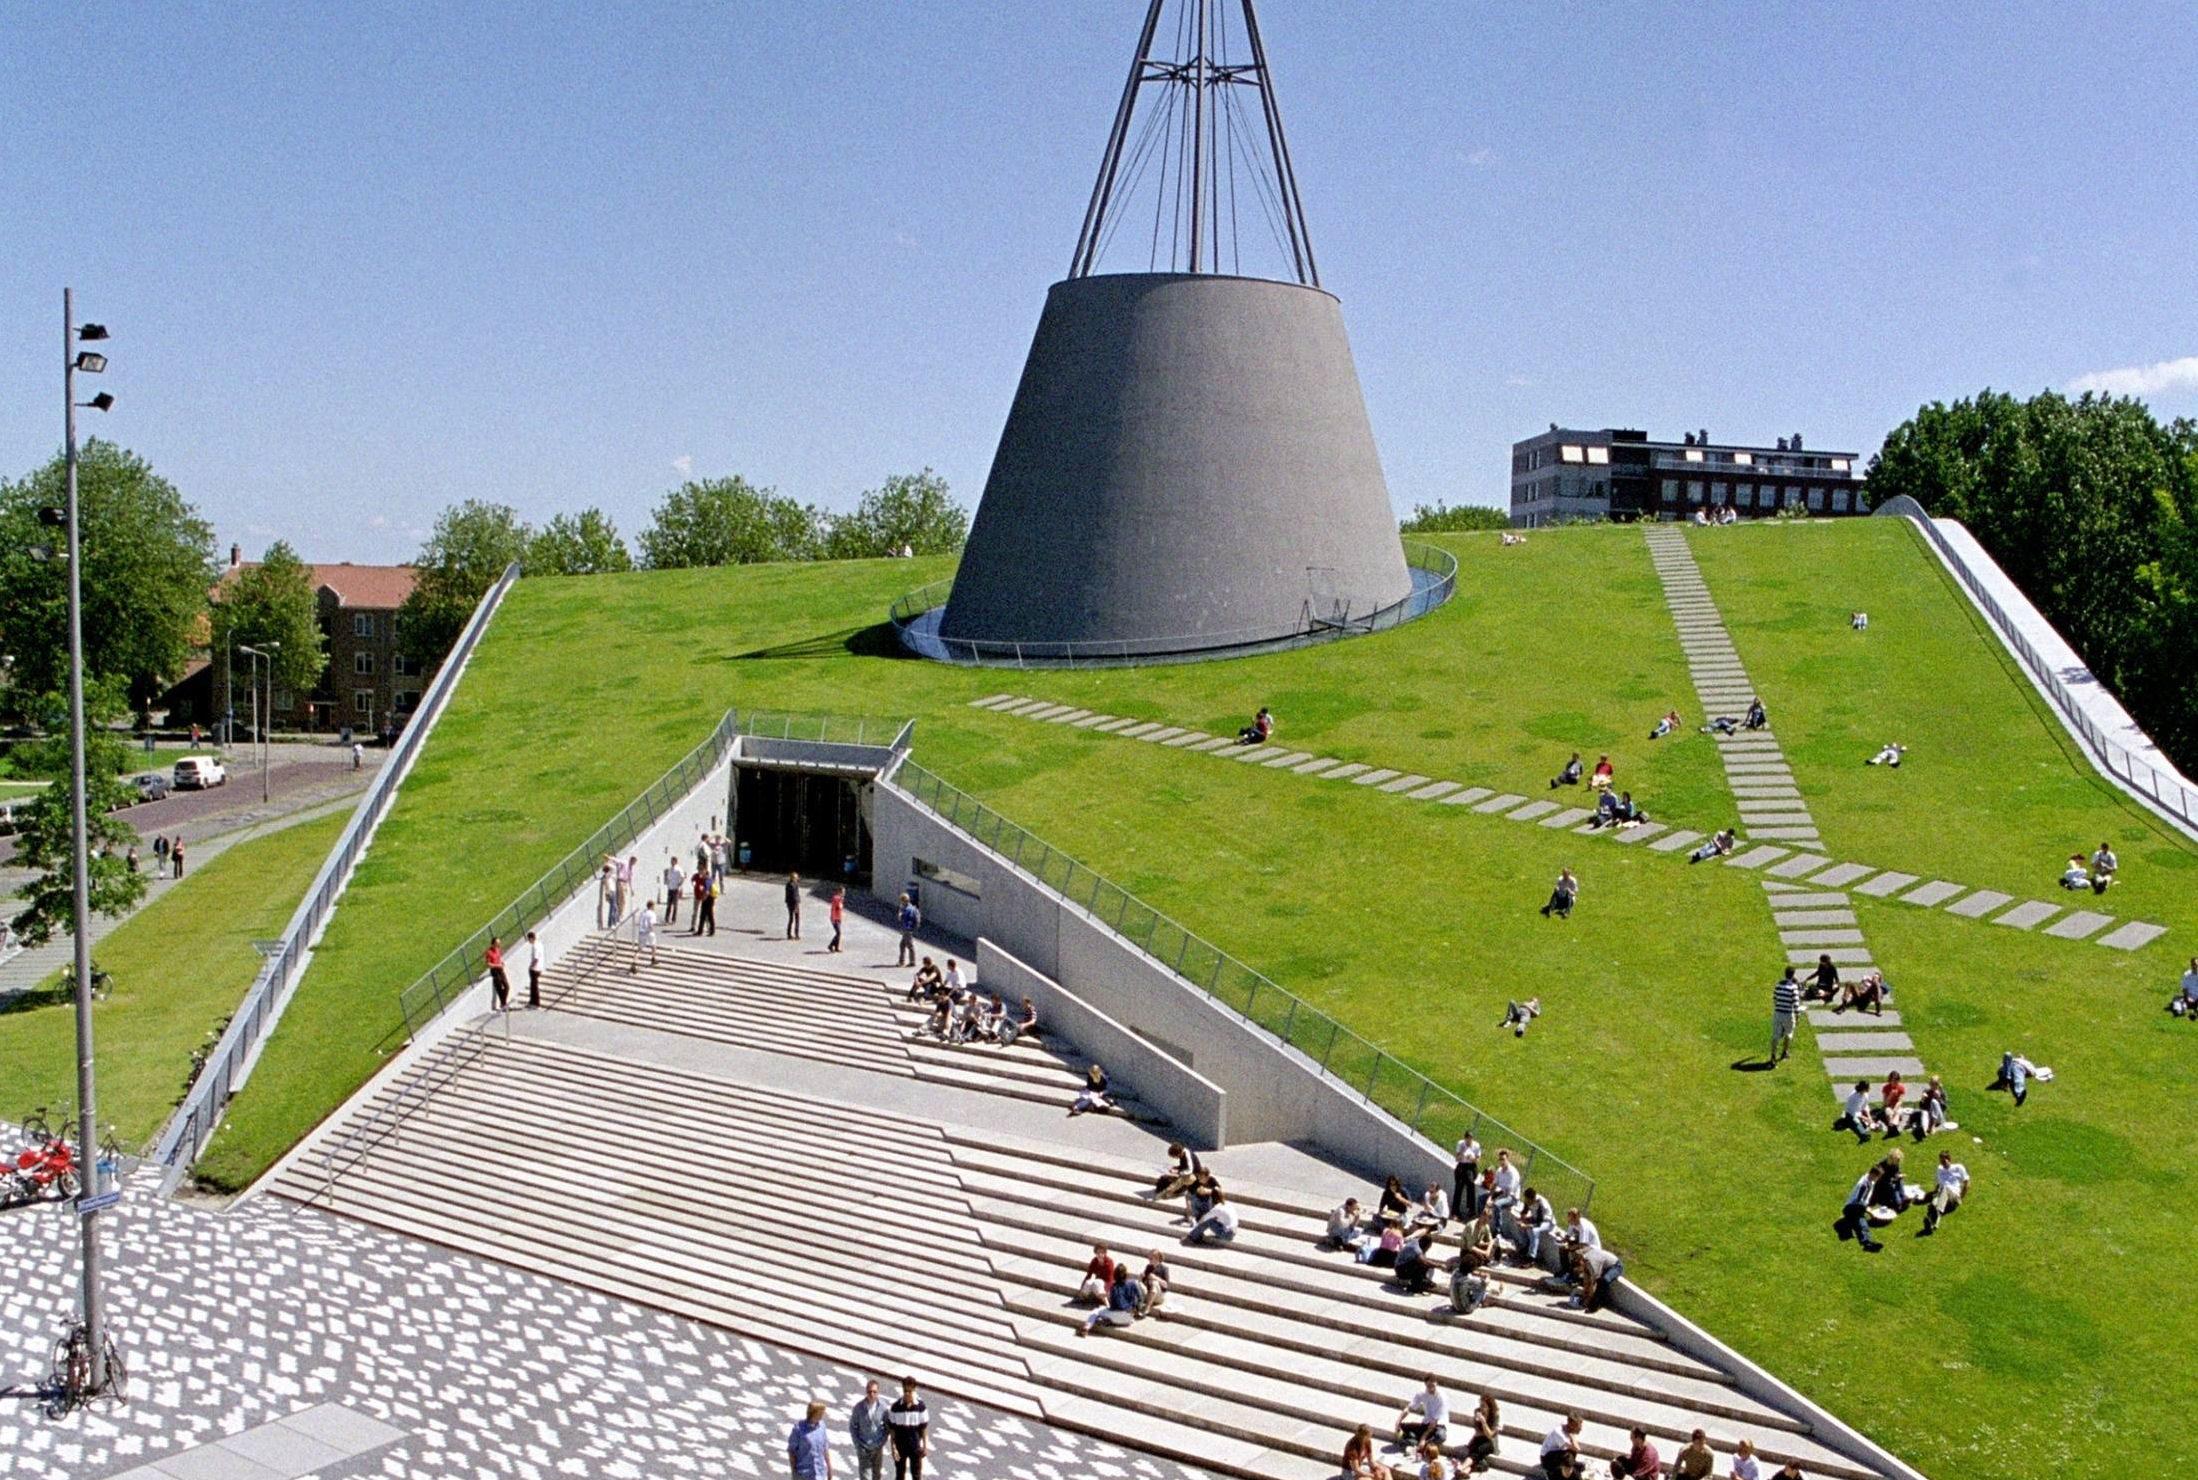
\includegraphics[height=8.65cm]{TUDelft/background-titlepage.jpg}}; % background photo
            {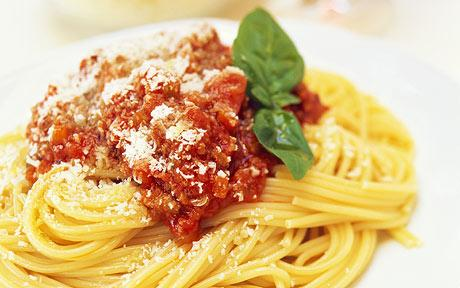
\includegraphics[height=8.65cm]{TUDelft/bolognese.jpg}}; % background photo
            \fill [cyan!95!black!70!blue] (0,2.9) -- (0,5.35) -- (-.5,5.35) -- (-.5,2.9) -- cycle ;%squareNorthWest
            \draw [fill=black] (0,0) -- (11,0) -- (11,2.9) -- (0,2.9) -- cycle ;
            \fill [fill=cyan!65!blue!80] (7,-3.9) -- (12.4,-3.9) -- (12.4,-3.65) -- (7,-3.65) -- cycle;
            \node [shift={(0.8cm,-2.9cm)},textlabel,right]  at (current page.north west) {\textbf{\LARGE{\textrm{\titel}}}};
            \node [shift={(0.8cm,-3.5cm)},textlabel,cyan!95!black!70!blue,right]  at (current page.north west)
            {\textbf{\large{\textrm{\subkop}}}};
            \node [shift={(0.8cm,-4.6cm)},textlabel,right]  at (current page.north west)
            {\normalsize{\naam}};
            \node [shift={(0.8cm,-5cm)},textlabel,right]  at (current page.north west)
            {\normalsize{\presentationdate}};
        \end{tikzpicture}};
    \end{tikzpicture}
\end{frame}


%--------------------------------------------
%%% Table of contents (TOC)
% The TOC will generated after building your section(s) and subsections
\begin{frame}<beamer>\frametitle{\textbf{\LARGE{\textrm{\titelTOC}}}}
    \begin{tikzpicture}[remember picture, overlay]
        \node [shift={(0.5 cm,-5.35cm)}]  at (current page.north west)
        {
        \begin{tikzpicture}[remember picture, overlay]
            \fill [fill=cyan!65!blue!80] (7,-3.9) -- (12.4,-3.9) -- (12.4,-3.65) -- (7,-3.65) -- cycle;
        \end{tikzpicture}};
    \end{tikzpicture}
    \tableofcontents
\end{frame}
%--------------------------------------------

\section{The Bologna process scheduling problem}
	\frame{\frametitle{Outline}\tableofcontents[currentsection,currentsubsection]}
\newpic{images/BPLogo.jpg}
\frame{\frametitle{The Bologna process scheduling problem}
	Parts of the problem:
	\begin{itemize}
		\item Modules
		\item Categories
		\item total ECTS
		\item (optimization goal)
	\end{itemize}
}
\nopic

\section{Our approach}
	\frame{\frametitle{Outline}\tableofcontents[currentsection]}
	
	\subsection{User interface with Flapjax}
	\frame{\frametitle{Outline}\tableofcontents[currentsection,currentsubsection]}
	\newpic{images/flapjacks.jpg}
	\frame{\frametitle{User interface with Flapjax}

	}
	\nopic

	\subsection{Constraint programming with OscaR}
	\frame{\frametitle{Outline}\tableofcontents[currentsection,currentsubsection]}
	\newpic{images/oscar.jpeg}
	\frame{\frametitle{Constraint programming with OscaR}
		\begin{itemize}
			\item Integer Programming
			\begin{itemize}
				\item decision variables per possible booking
				\item never double book a Module
				\item book at least Category.min ECTS
				\item obtain enough \emph{creditable} ECTS
			\end{itemize}

			\item Encapsulating side-effects
			\begin{itemize}
				\item AST as constraint model
				\item the OscaR monad
			\end{itemize}
		\end{itemize}
	}
	\nopic

\section{What we learned}
	\frame{\frametitle{Outline}\tableofcontents[currentsection,currentsubsection]}
	\newpic{images/binary.jpg}
	\frame{\frametitle{What we learned}
		\begin{tikzpicture}
			\node at (0,1.5)
			{
\includegraphics[width=3cm]{images/oscarlogo.png}};
			\node at (0,0)
			{
\includegraphics[width=3cm]{images/scalaLogo.png}};
			\node at (0,-1.0)
			{
\includegraphics[width=3cm]{images/flapjaxlogo.png}};
			\node at (0,-2.5)
			{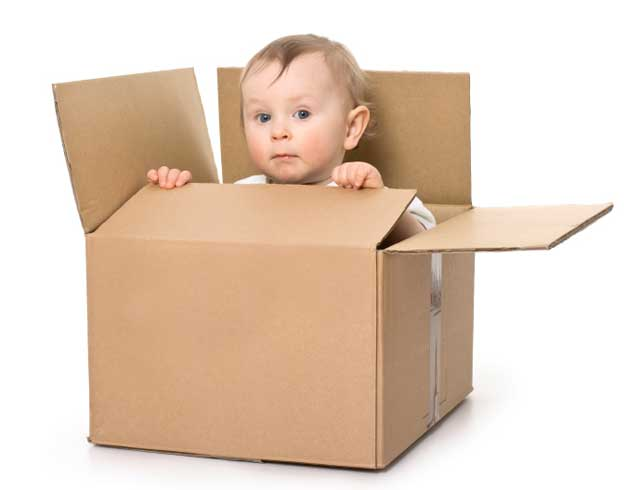
\includegraphics[width=3cm]{images/monad.jpg}};
			\node at (-0.43,-3.0){Monads};
		\end{tikzpicture}
	}
	\nopic

\section{Demo}
	\frame{\frametitle{Outline}\tableofcontents[currentsection,currentsubsection]}

\section{Questions}
	\frame{\frametitle{Outline}\tableofcontents[currentsection,currentsubsection]}

\end{document} 
